%%%%%%%%%%%%%%%%%%%%%%%%%%%%%%%%%%%%%%%%%%%%%%%%%%%%%%%%%%%%%%%%%%%%%
% LaTeX Template: Project Titlepage Modified (v 0.1) by rcx
%
% Original Source: http://www.howtotex.com
% Date: February 2014
% 
% This is a title page template which be used for articles & reports.
% 
% This is the modified version of the original Latex template from
% aforementioned website.
% 
%%%%%%%%%%%%%%%%%%%%%%%%%%%%%%%%%%%%%%%%%%%%%%%%%%%%%%%%%%%%%%%%%%%%%%

\documentclass[12pt]{report}
\usepackage[a4paper]{geometry}
\usepackage[myheadings]{fullpage}
\usepackage{fancyhdr}
\usepackage{lastpage}
\usepackage{graphicx, wrapfig,setspace, booktabs}
\usepackage[T1]{fontenc}
\usepackage[font=small, labelfont=bf]{caption}
\usepackage{fourier}
\usepackage[protrusion=true, expansion=true]{microtype}
\usepackage[english]{babel}
\usepackage{sectsty}
\usepackage{lipsum}
\usepackage[hyphens]{url}
%\usepackage{subfig}
\usepackage{hyperref}
\usepackage{alphalph}
\usepackage[utf8]{inputenc}
\usepackage{multicol}
\usepackage{amsmath}
\usepackage{subfigure}
\renewcommand*{\thesubfigure}{%
\alphalph{\value{subfigure}}%
}%


\newcommand{\HRule}[1]{\rule{\linewidth}{#1}}
\onehalfspacing
\setcounter{tocdepth}{5}
\setcounter{secnumdepth}{5}
\usepackage{float}

\usepackage[backend=bibtex,style=chem-acs,biblabel=dot]{biblatex}
\addbibresource{references.bib}

%-------------------------------------------------------------------------------
% HEADER & FOOTER
%-------------------------------------------------------------------------------
\pagestyle{fancy}
\fancyhf{}
\setlength\headheight{15pt}
\fancyhead[L]{CS7015: PA4}
\fancyhead[R]{Deep Learning}
\fancyfoot[R]{Page \thepage\ of \pageref{LastPage}}
%-------------------------------------------------------------------------------
% TITLE PAGE
%-------------------------------------------------------------------------------

\begin{document}

\title{ \normalsize \textsc{CS7015 : Deep Learning}
		\\ [2.0cm]
		\HRule{0.5pt} \\
		\LARGE \textbf{\uppercase{Programming Assignment 4}}\\
        \large{- seq2seq LSTM with Attention -}
		\HRule{2pt} \\ [0.5cm]
		\normalsize \today \vspace*{5\baselineskip}}

\date{}

\author{
		Student ID:  \\ 
		Namida M - EE15B123 \\
		Ganga Meghanath - EE15B025
		}

\renewcommand\thesection{\arabic{section}}
\maketitle
\tableofcontents
\newpage

%-------------------------------------------------------------------------------
% Section title formatting
\sectionfont{\scshape}
%-------------------------------------------------------------------------------

%-------------------------------------------------------------------------------
% BODY
%-------------------------------------------------------------------------------

\section{Introduction}
Weather Gov Data
%-------------------------------------------------------------------------------
%DATA ANALYSIS
%-------------------------------------------------------------------------------
\section{Mathematical formulation}
Write down the mathematical formulation for both Basic Encoder and Hierarchical Encoder. i.e given the Source Table as a collection of Field words {f1, f2, ..., fn} where each field contains {w1f , w2f , ...., wmf } tokens. Write the step by steps trans- formations done to reach the text description Y which is basically a sequence of words {y1, y2, ..., yk}.\\

\subsection{Basic encoder}
A single LSTM is used for encoding : 
\[
h^w_t = LSTM_{encode}^{word}(e^w_t, h^w_{t-1})
\]
The vector output at the ending time is used to represent the entire table : 
\[
e_T = h^w_{T}
\]
The final state is passed to the decoder.

\subsection{Attention mechanism on top of a Basic encoder}
A single LSTM is used for encoding : 
\[
h^w_t = LSTM_{encode}^{word}(e^w_t, h^w_{t-1})
\]
The vector output at the ending time is used to represent the entire table : 
\[
e_T = h^w_{T}
\]
Implementing Attention over the LSTM,
$$e_{jt} = V_{Att}^T \ tanh(U_{Att} \ h^w_j + W_{Att} \ s_t + b_{Att}) $$
$$\alpha_{jt} = softmax(e_{jt})$$
$$c_t = \sum_{j=1}^T \alpha_{jt} h^w_j$$
The final state is passed to the decoder as $[e_T, c_t]$.

\subsection{Hierarchical encoder}
A layer of LSTM is placed on top of the words in a sentence :
\[
h^w_t = LSTM_{encode}^{word}(e^w_t, h^w_{t-1})
\]
The vector output at the ending time is used to represent the entire sentence : 
\[
e_s = h^w_{T}
\]
Another layer of LSTM is placed on top of all sentences :
\[
s^s_t = LSTM_{encode}^{sentence}(e^s_t, s^s_{t-1})
\]
Hence, the entire document(table) is represented by :
\[
e_{table} = s^s_T
\]
The final state is passed to the decoder.

\subsection{Attention mechanism on top of a Hierarchical encoder}
A layer of LSTM is placed on top of the words in a sentence :
\[
h^w_t = LSTM_{encode}^{word}(e^w_t, h^w_{t-1})
\]
The vector output at the ending time is used to represent the entire sentence : 
\[
e_s = h^w_{T}
\]
Implementing Attention over the LSTM over words,

$$e^w_{jt} = (V^w_{Att})^T \ tanh(U^w_{Att} \ h^w_j + W^w_{Att} \ h^s_t + b^w_{Att}) $$
$$\alpha^w_{jt} = softmax(e^w_{jt})$$
$$c^w_t = \sum_{j=1}^T \alpha^w_{jt} h^w_j$$
Another layer of LSTM is placed on top of all sentences :
\[
h^s_t=LSTM_{encode}^{sentence}([e^s_t,c^w_t], h^s_{t-1})
\]
Hence, the entire document(table) is represented by :
\[
e_{table} = s^s_T
\]
Implementing Attention over the LSTM over sentences,

$$e_{jt} = V_{Att}^T \ tanh(U_{Att} \ h^s_j + W_{Att} \ s_t + b_{Att}) $$
$$\alpha_{jt} = softmax(e_{jt})$$
$$c_t = \sum_{j=1}^T \alpha_{jt} h^s_j$$
The final state is passed to the decoder as $[e_{table}, c_t]$.

\section{Plots of training and validation loss}

\subsection{Basic encoder-decoder}
\begin{center}
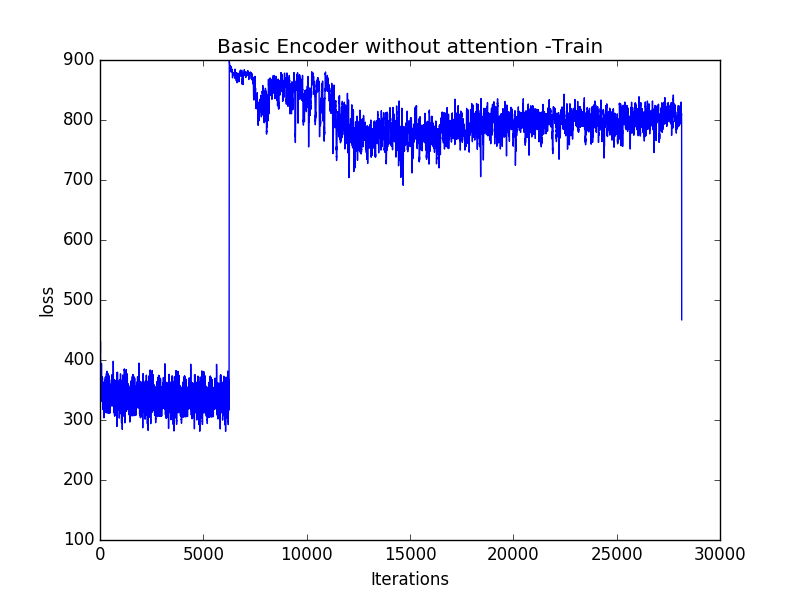
\includegraphics[scale=0.5]{train_basic.png}
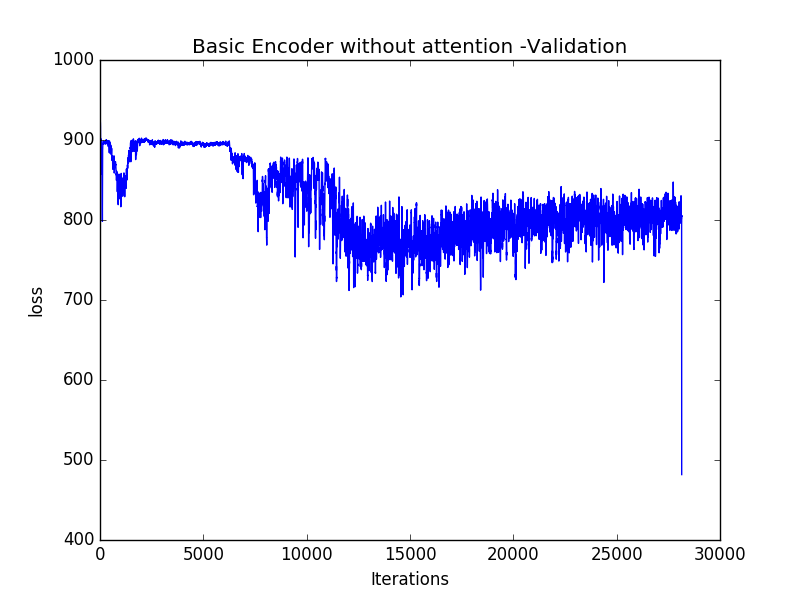
\includegraphics[scale=0.5]{val_basic.png}
\end{center}

\subsection{Basic encoder-decoder with attention mechanism}
The tensorflow scalars generated for training is as follows :
\\For a learning rate of 0.0001 and Adam optimizer
\begin{center}
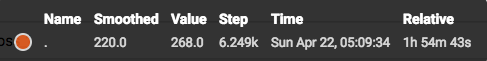
\includegraphics[scale=0.5]{lr_0_0001_attn_train_25k_result.png} \\
\vspace{3mm}
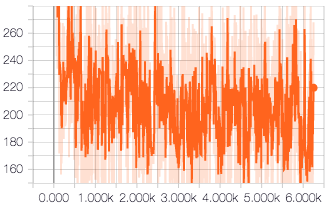
\includegraphics[scale=0.6]{lr_0_0001_attn_train_25k.png}\\
\vspace{3mm}

\includegraphics[scale=0.5]{lr_0_0001_attn_greedy_25k_result.png} \\
\vspace{3mm}
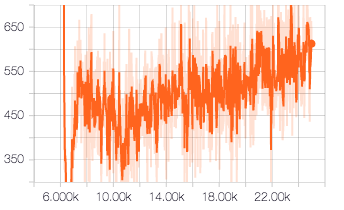
\includegraphics[scale=0.6]{lr_0_0001_attn_greedy_25k.png} 
\end{center}
For a learning rate of 0.001 and Adam optimizer
\begin{center}

\includegraphics[scale=0.5]{lr_0_001_attn_train_25k_result.png} \\
\vspace{3mm}
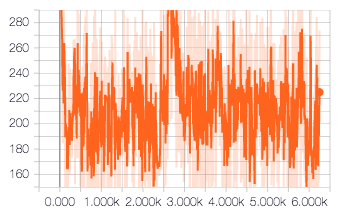
\includegraphics[scale=0.6]{lr_0_001_attn_train_25k.png}\\
\vspace{3mm}
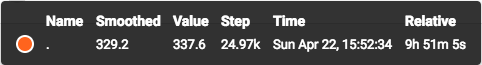
\includegraphics[scale=0.5]{lr_0_001_attn_greedy_25k_result.png} \\
\vspace{3mm}
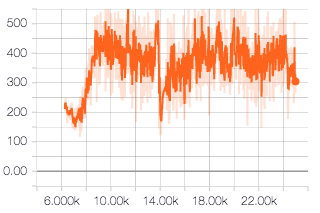
\includegraphics[scale=0.7]{lr_0_001_attn_greedy_25k.png} 
\end{center}
 
The training and validation loss plotted in python has been shown below :
\\For a learning rate of 0.0001 and Adam optimizer
\begin{center}
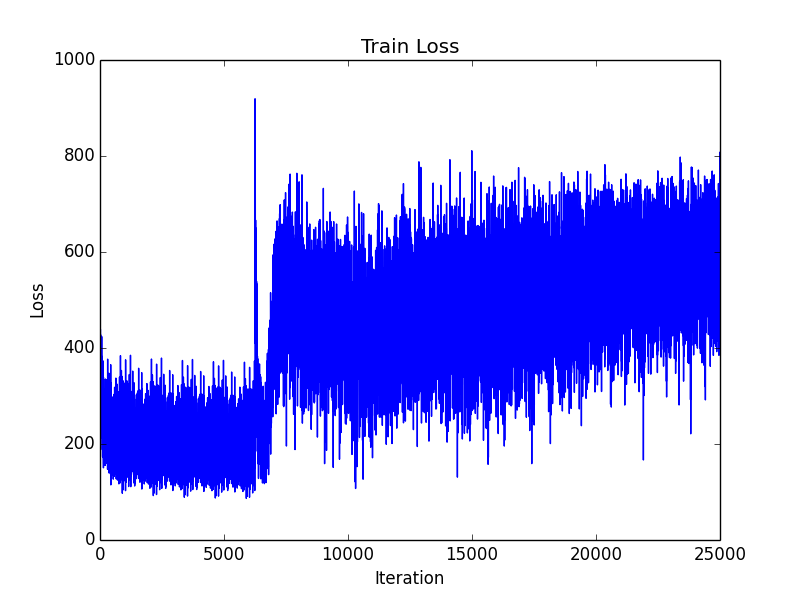
\includegraphics[scale=0.5]{train_loss1.png} \\
\vspace{3mm}
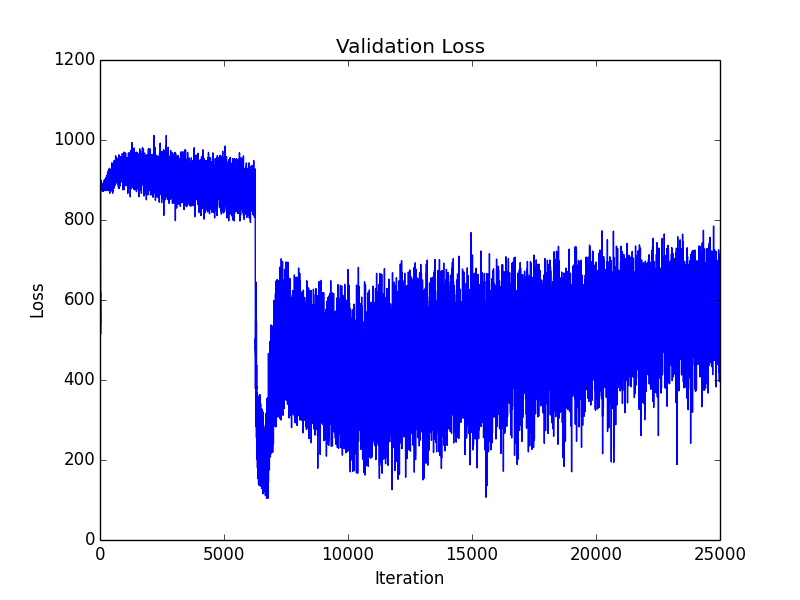
\includegraphics[scale=0.5]{val_loss1.png} 
\end{center}
For a learning rate of 0.001 and Adam optimizer
\begin{center}
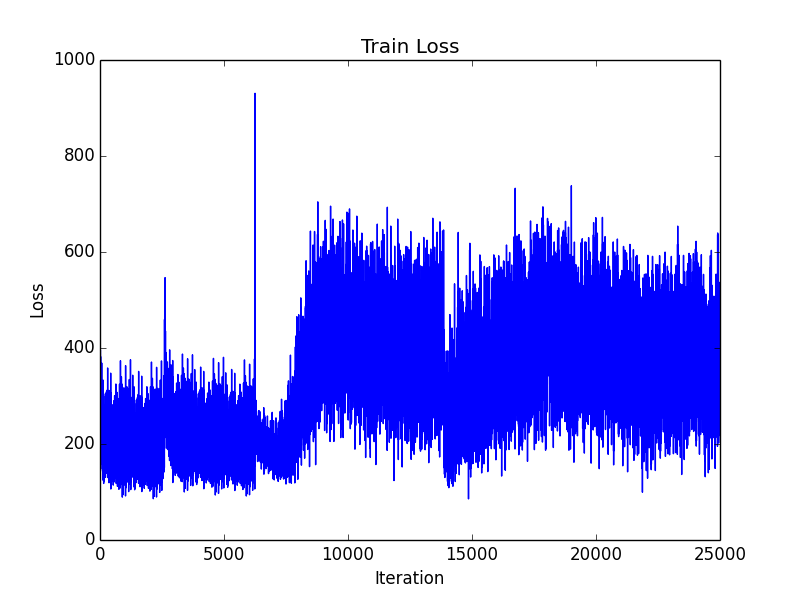
\includegraphics[scale=0.5]{train_loss2.png} \\
\vspace{3mm}
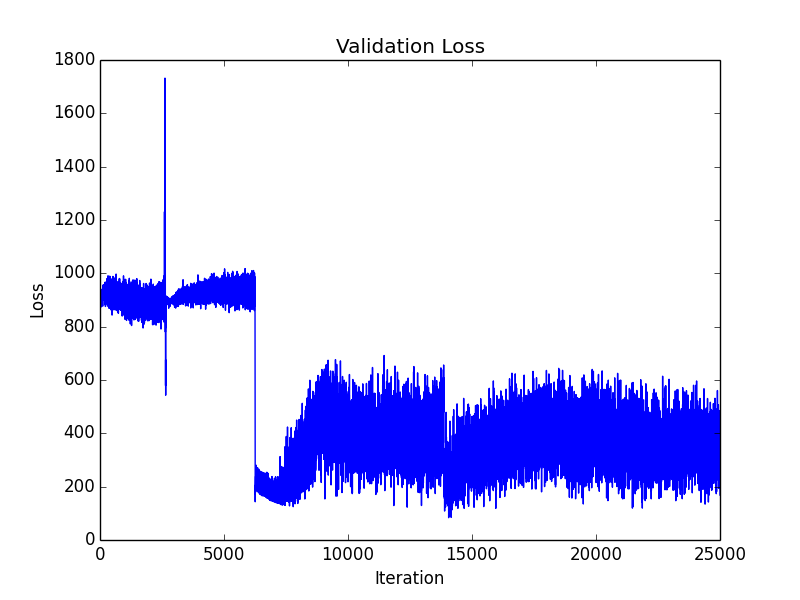
\includegraphics[scale=0.5]{valid_loss2.png} 
\end{center}

\section{Models}
\subsection{Best Model}
The best model was found to be using Basic encoder with Attention. The training was stopped when the validation error was minimum, and this was found out through early stopping and the model with the least validation score was restored.
\subsubsection{Parameter setting}
For a learning rate of 0.001 and Adam optimizer, the algorithm was run for 8750 iterations (1250 iterations = 1 epoch)
\begin{center}
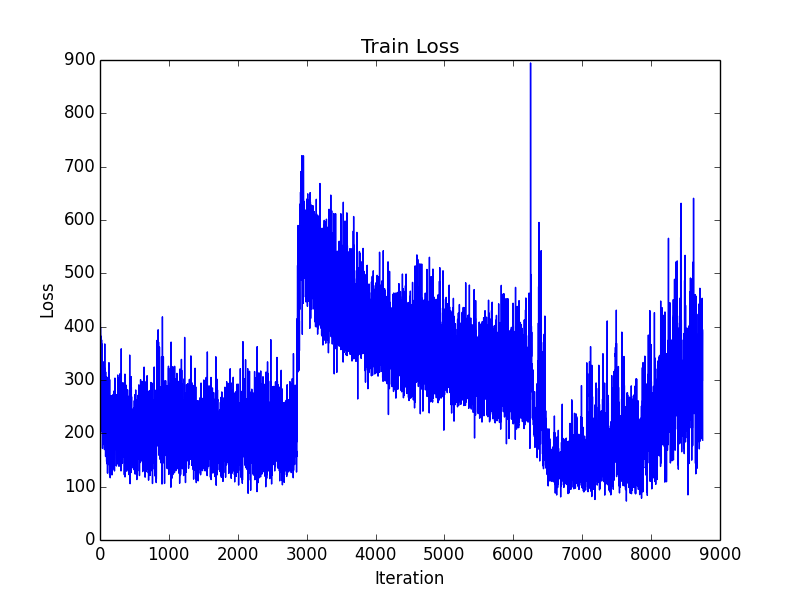
\includegraphics[scale=0.5]{train_loss_8500.png} \\
\vspace{3mm}
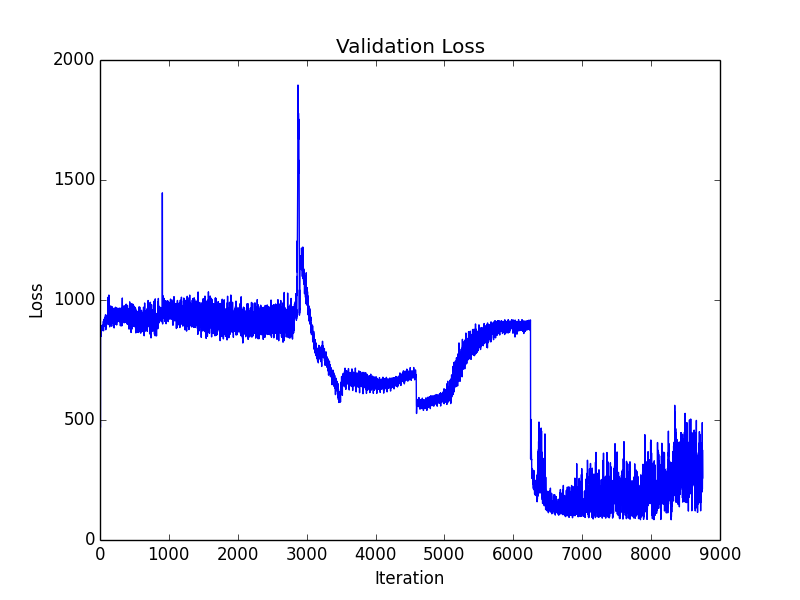
\includegraphics[scale=0.5]{val_loss_8500.png} 
\end{center}
\subsubsection{Performance}
The model gave a validation score of 295.8670654296875 for the entire validation set at the end of training.
\\
\subsection{Model 1 : Basic encoder-decoder}
Configuration details :
\begin{table}[H]
	\label{T:equipos}
	\begin{center}
		\begin{tabular}{| c | c | c | c | c | c |}
			\hline
			\textbf{Layer} & \textbf{Input Shape} & \textbf{Output Shape}\\ 
			\hline
			INEMBED & (20 × max$\_$index(batch))& ((20 × max$\_$index(batch) x 100) \\
            ENCODER & ((20 × max$\_$index(batch) x 100) & (20 × 512) \\
            DECODER & (20 x 150 x 512) & (20 x 150 x 512) \\
            SOFTMAX  & (20 x 150 x 512) & (20 x 150 x 512) \\
            OUTEMBED  & (20 x 150 x 512) & (20 x 150 x 512) \\
            \hline
		\end{tabular}
	\end{center}
\end{table}
The encoder is a bidirectional RNN with forward and backward cell size as 512. So, when passing the final state to the decoder , we have to concatenate the states. We have chosen to project the states to the decoder.\\So, the output from the encoder is an LSTM state tuple of the form $(c_{fw},h_{fw}),(c_{bw},h_{bw})$.\\\\

\textbf{SOME TEST SUMMARIES}
\begin{itemize}
\item partly sunny , with a high near 80 . breezy , with a south wind between 11 and 21 mph .
\item showers , with thunderstorms also possible after 10pm . low around 38 . south wind wind around and mph mph . chance of precipitation is is $\%$ . .
\end{itemize}


\subsection{Model 3 : Basic encoder-decoder with Attention mechanism}
Configuration details :
\begin{table}[H]
	\label{T:equipos}
	\begin{center}
		\begin{tabular}{| c | c | c | c | c | c |}
			\hline
			\textbf{Layer} & \textbf{Input Shape} & \textbf{Output Shape}\\ 
			\hline
			INEMBED & (20 × max$\_$index(batch))& ((20 × max$\_$index(batch) x 100) \\
            ENCODER & ((20 × max$\_$index(batch) x 100) & (20 × 512) \\
            DECODER & (20 x 150 x 512) & (20 x 150 x 512) \\
            SOFTMAX  & (20 x 150 x 512) & (20 x 150 x 512) \\
            OUTEMBED  & (20 x 150 x 512) & (20 x 150 x 512) \\
            \hline
		\end{tabular}
	\end{center}
\end{table}
The dimensions remain the same as in the case of a basic decoder without attention.
Here, instead of passing the final state, we pass a weighted sum of the weights, over the time steps.\\\\
\textbf{SOME TEST SUMMARIES}
\begin{itemize}
\item A 20 percent chance of showers . mostly cloudy , with a with a near . . wind wind wind and with with mph as high as
\item Mostly cloudy , with a low around . . south wind between 5 and 15 mph . 
\end{itemize}

\section{Analysis}

\subsection{Effect of using unidirectional LSTM for the encoder}
The performance of the encoder-decoder model using a uni-directional LSTM is not as good as in the case of a bidirectional LSTM, as the state only captures past context, not (future context).

The learning curves are as follows:
\begin{center}
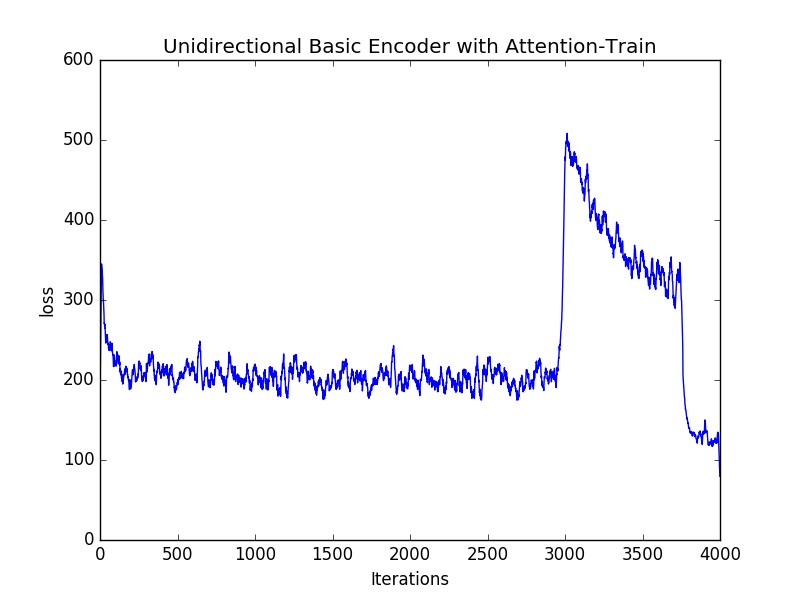
\includegraphics[scale=0.5]{uni_basic_train.png}
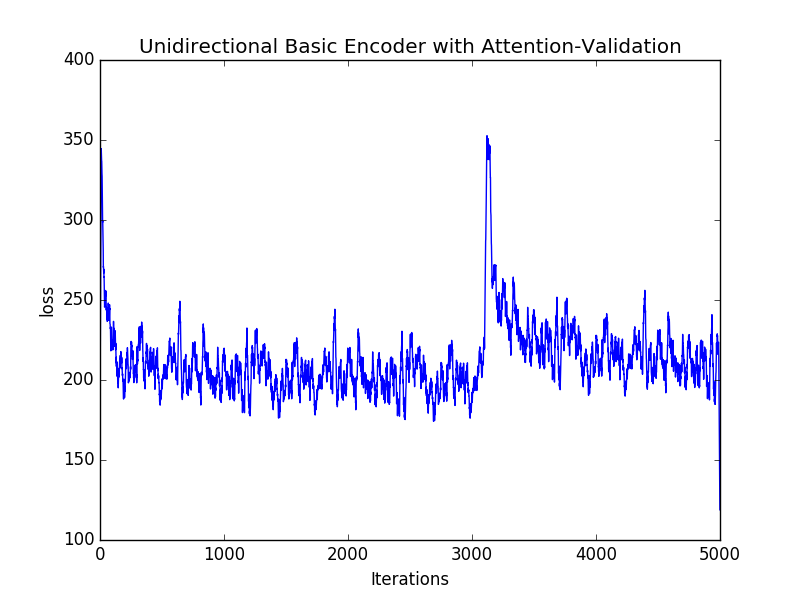
\includegraphics[scale=0.5]{uni_basic_val.png}
\end{center}
\textbf{SOME TEST SUMMARIES}
\begin{itemize}
\item Increasing clouds , with a low around . . wind wind between and wind and mph mph . 
\item A chance of rain before before . cloudy . cloudy . cloudy , a , a , a , a . . . . . . . . . . 
 
\end{itemize}
\subsection{Basic vs Hierarchical Encoder (Without Attention)}
The Hierarchical encoder should ideally perform better, as the basic encoder without attention, doesnt know which part of the table is important, while the Hierarchical encoder by structure is made to pay attention to the respective part of table.

\subsection{Effect of using Attention mechanism}
Introducing attention mechanism to the model causes an improvement in performance. Naturally, when summarizing a table we tend to focus on different aspects of the data as we write our summmary. 
In case of a basic encoder, the model has to learn how each row corresponds to an attribute, and within each row ,it needs to learn to focus as different aspects of that attribute.\\
For the hierarchical encoder, the model will learn how to pay attention to different parts of a row(on the first level), and then, over the rows. 

\subsection{Optimality of early stopping}
On running for 20 epochs, the results were obtained as follows :\\\\
For a learning rate of 0.0001 and Adam optimizer
\begin{center}
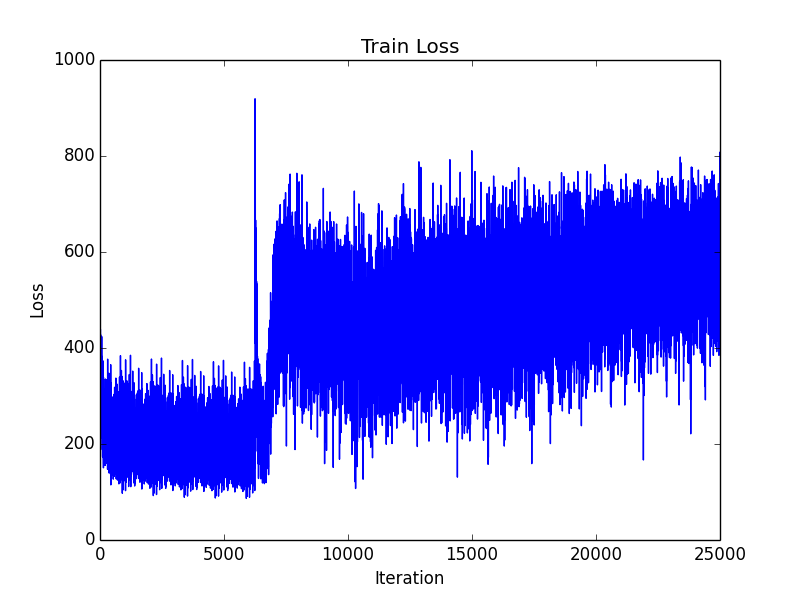
\includegraphics[scale=0.5]{train_loss1.png} \\
\vspace{3mm}
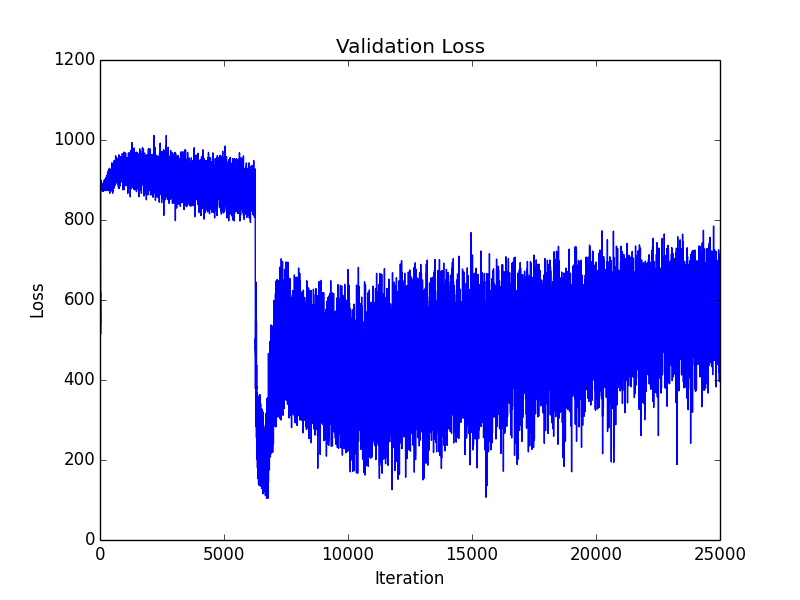
\includegraphics[scale=0.5]{val_loss1.png} 
\end{center}
In this case, on an average, the validation loss doesn't look like it's going to decrease after running it for epochs beyond the early stopping criterion. We can see that, on an average, the loss seems to be increasing. But since we use the model that gives the lowest validation loss, we see that after the first minima, the graph on an average goes up and then the loss decreases again to around the minimal value and then seems to increase. At the same time, train loss also increases. Hence, had we run it for a lot more epochs, there may come a point which is more optimal. LSTMs have a large number of parameters that need to be trained. Hence we cannot state anything solid.\\

For a learning rate of 0.001 and Adam optimizer
\begin{center}
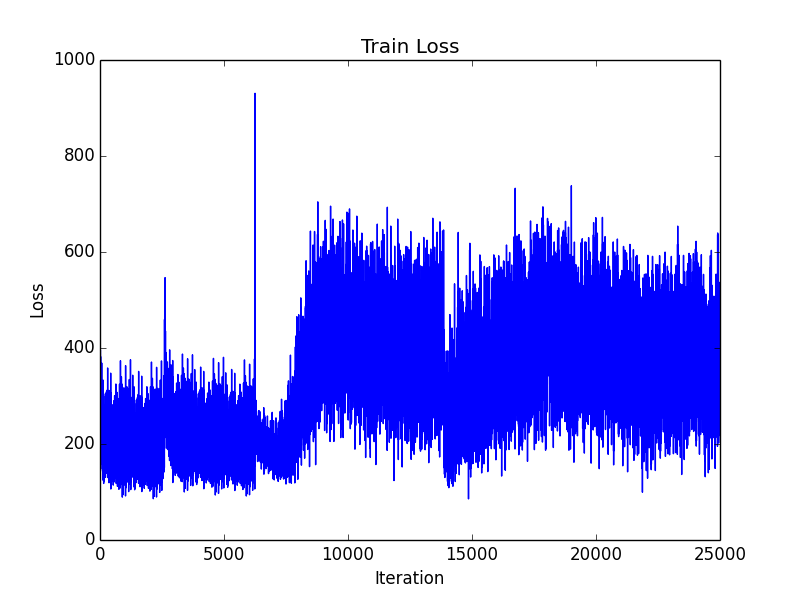
\includegraphics[scale=0.5]{train_loss2.png} \\
\vspace{3mm}
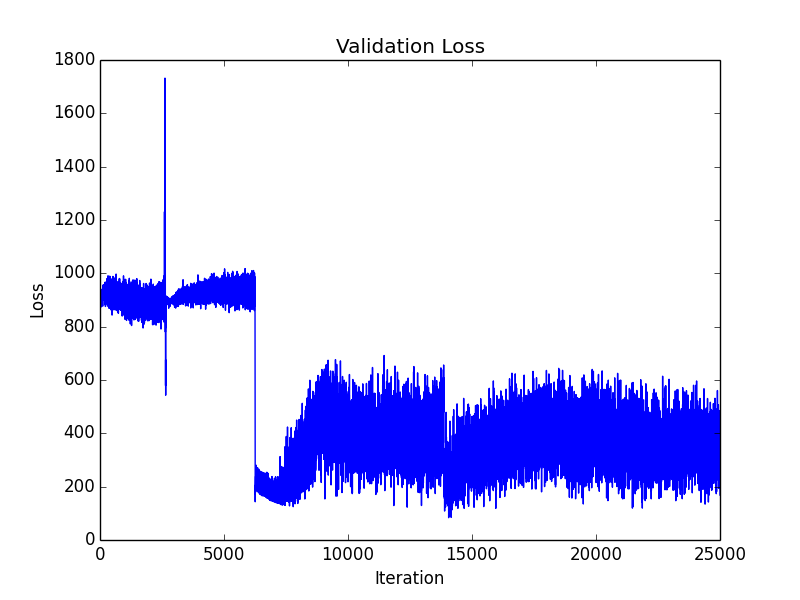
\includegraphics[scale=0.5]{valid_loss2.png} 
\end{center}
Here both the training and validation loss seems to be decreasing after a couple of epochs from the stopping criterion used from early stopping. Hence had we continued training, we might have been able to find a pint of minima which is more  optimal that the one given by the early stopping criterion.\\\\
Google colab allocates a GPU for 12 hours and that is enough only for 20 epochs and hence we didn't get a chance to explore further. Although we did try downloading the saved model, it gave a timeout error.
\subsection{Visualization of Attention layer weights for a sequence pair}
\begin{center}
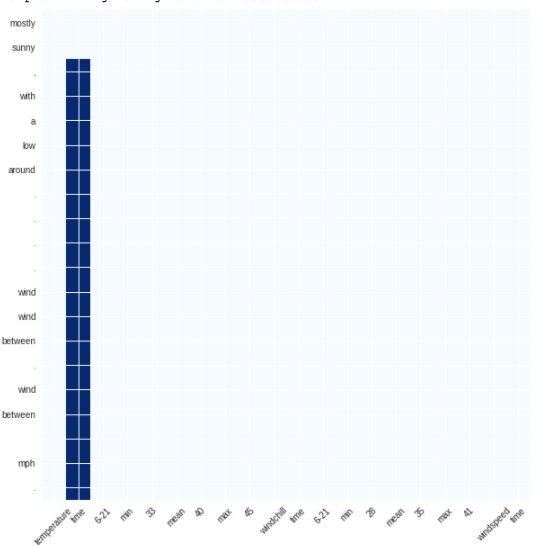
\includegraphics[scale=0.5]{pic2.png}
\end{center}
Unable to train for meaningful model due to time constraints, and runtime disconnect on google colab
\section{Appendix}
\subsection{Main Graph}
\begin{center}
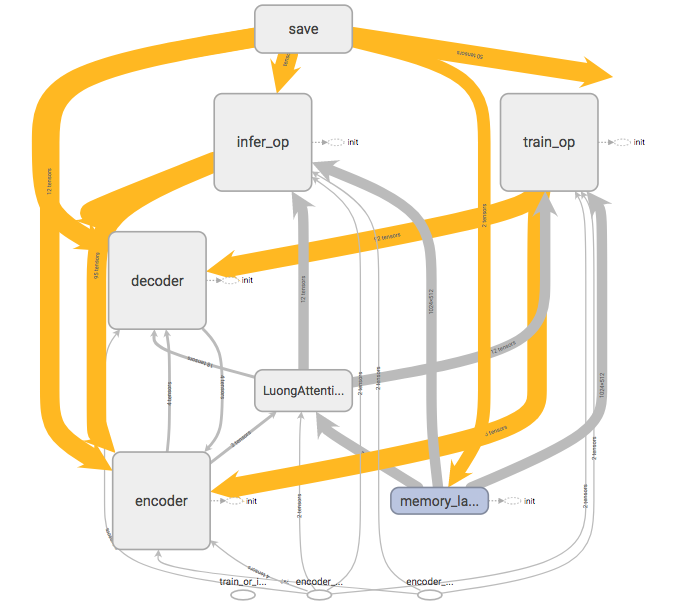
\includegraphics[scale=0.7]{Main_graph.png}
\end{center}

%-------------------------------------------------------------------------------
% REFERENCES
%-------------------------------------------------------------------------------
\begin{thebibliography}{9}
\bibitem{1} 
Mitesh M Khapra. \textit{CS7015 Deep Learning: Lecture 13-18}, 
Indian Institute of Technology Madras, 2018
\end{thebibliography}


\end{document}

%-------------------------------------------------------------------------------
% SNIPPETS
%-------------------------------------------------------------------------------

%\begin{figure}[!ht]
%	\centering
%	\includegraphics[width=0.8\textwidth]{file_name}
%	\caption{}
%	\centering
%	\label{label:file_name}
%\end{figure}

%\begin{figure}[!ht]
%	\centering
%	\includegraphics[width=0.8\textwidth]{graph}
%	\caption{Blood pressure ranges and associated level of hypertension (American Heart Association, 2013).}
%	\centering
%	\label{label:graph}
%\end{figure}

%\begin{wrapfigure}{r}{0.30\textwidth}
%	\vspace{-40pt}
%	\begin{center}
%		\includegraphics[width=0.29\textwidth]{file_name}
%	\end{center}
%	\vspace{-20pt}
%	\caption{}
%	\label{label:file_name}
%\end{wrapfigure}

%\begin{wrapfigure}{r}{0.45\textwidth}
%	\begin{center}
%		\includegraphics[width=0.29\textwidth]{manometer}
%	\end{center}
%	\caption{Aneroid sphygmomanometer with stethoscope (Medicalexpo, 2012).}
%	\label{label:manometer}
%\end{wrapfigure}

%\begin{table}[!ht]\footnotesize
%	\centering
%	\begin{tabular}{cccccc}
%	\toprule
%	\multicolumn{2}{c} {Pearson's correlation test} & \multicolumn{4}{c} {Independent t-test} \\
%	\midrule	
%	\multicolumn{2}{c} {Gender} & \multicolumn{2}{c} {Activity level} & \multicolumn{2}{c} {Gender} \\
%	\midrule
%	Males & Females & 1st level & 6th level & Males & Females \\
%	\midrule
%	\multicolumn{2}{c} {BMI vs. SP} & \multicolumn{2}{c} {Systolic pressure} & \multicolumn{2}{c} {Systolic Pressure} \\
%	\multicolumn{2}{c} {BMI vs. DP} & \multicolumn{2}{c} {Diastolic pressure} & \multicolumn{2}{c} {Diastolic pressure} \\
%	\multicolumn{2}{c} {BMI vs. MAP} & \multicolumn{2}{c} {MAP} & \multicolumn{2}{c} {MAP} \\
%	\multicolumn{2}{c} {W:H ratio vs. SP} & \multicolumn{2}{c} {BMI} & \multicolumn{2}{c} {BMI} \\
%	\multicolumn{2}{c} {W:H ratio vs. DP} & \multicolumn{2}{c} {W:H ratio} & \multicolumn{2}{c} {W:H ratio} \\
%	\multicolumn{2}{c} {W:H ratio vs. MAP} & \multicolumn{2}{c} {\% Body fat} & \multicolumn{2}{c} {\% Body fat} \\
%	\multicolumn{2}{c} {} & \multicolumn{2}{c} {Height} & \multicolumn{2}{c} {Height} \\
%	\multicolumn{2}{c} {} & \multicolumn{2}{c} {Weight} & \multicolumn{2}{c} {Weight} \\
%	\multicolumn{2}{c} {} & \multicolumn{2}{c} {Heart rate} & \multicolumn{2}{c} {Heart rate} \\
%	\bottomrule
%	\end{tabular}
%	\caption{Parameters that were analysed and related statistical test performed for current study. BMI - body mass index; SP - systolic pressure; DP - diastolic pressure; MAP - mean arterial pressure; W:H ratio - waist to hip ratio.}
%	\label{label:tests}
%\end{table}